%% 歩容パターンの再評価手法の実装.tex
%% LaTeX-2e 専用

\chapter{歩容パターンの再評価手法の実装}\label{chapter:歩容パターンの再評価手法の実装}
第\ref{chapter:歩容パターンの再評価手法の実装}章では,
第\ref{chapter:歩容パターンの再評価手法の提案}章で述べた歩容パターンの再評価手法の実装方法について述べる.

\section{グラフ探索による自由歩容パターン生成手法の実装}
再評価手法の実装方法の説明の前に,グラフ探索による自由歩容パターン生成手法の実装方法について述べる.
波東らが用いたグラフ探索による自由歩容パターン生成手法と同様の手法によって歩容パターンを生成しているが,
より早い処理の実現やプログラムの可読性・拡張性の向上のため,その実装方法を1部変更している.
加えて,新たに3次元不整地における旋回動作の実装を行ったため,改めて実装方法を説明する.
実装はC++20を用いて行っており,命名規則はGoogle~C++~Style~Guide\cite{cita:google_cpp_style_guide}にしたがっている.
また,この章におけるクラスや構造体の図はUML(Unified~Modeling~Language)を用いて表現されており,
上からクラス・構造体の名前,メンバ変数,メンバ関数を表している.
メンバ変数は,アクセス修飾子,変数名,型の順に記述されており,
メンバ関数は,アクセス修飾子,関数名,引数,戻り値の順に記述されている.
アクセス修飾子は記号を用いて表し,+はpublic,protectedは\#,
privateは$-$である.

\subsection{プログラム全体の流れ}
グラフ探索による自由歩容パターン生成手法では,
歩容パターングラフの作成,歩容パターングラフの探索の2つの処理を行う.
歩容パターングラフを作成する処理はGraphTreeCreatorクラスで実装されており,
歩容パターングラフの探索を行う処理はGraphSearcherクラスで実装されている.

これらの処理の流れを\figref{fig:graph_search_sequence}に示す.
まず,GraphTreeCreatorクラスに現在のロボットの状態を表すノードを渡す.
GraphTreeCreatorクラスは,渡されたノードを根ノードとする歩容パターングラフを作成する.
次に,GraphSearcherクラスに作成された歩容パターングラフを渡す.
このとき,値をコピーして渡すのではなく,
ポインタを渡すことでメモリの使用量を削減するとともに,
グラフ探索の処理時間を短縮している.
GraphSearcherクラスは,渡された歩容パターングラフを探索し,
最適な歩容パターンを見つけ,その歩容パターンを返す.
以上の流れでグラフ探索による自由歩容パターン生成手法を実装している.



\begin{figure}[htbp]
  \begin{center}
    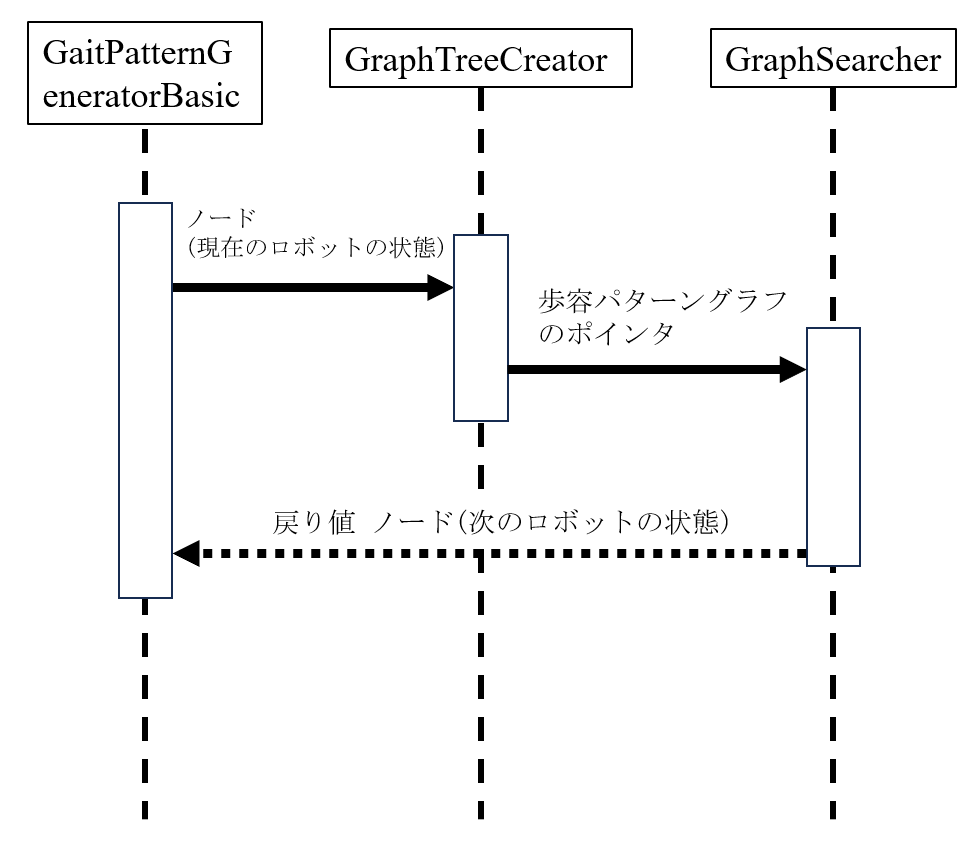
\includegraphics[width=75mm, clip]{figure/chapter3/sequence_main.png}
    \caption{Graph Search Sequence}
    \label{fig:graph_search_sequence} % chktex 24
  \end{center}
\end{figure}

\begin{figure}[htbp]
  \centering
  \begin{tikzpicture}[show background grid]
    \begin{interface}[text width=10mm]{IGaitPatternGenerator}{-12, -4}
      \attribute{}
      \operation{+ GetNextNodeByGraphSearch() }
    \end{interface}

    \begin{class}[text width=70mm]{GaitPatternGeneratorBasic}{-12, 0}
      \inherit{IGaitPatternGenerator}
      \attribute{- graph\_searcher\_ptr\_ : std::unique\_ptr\textless~IGraphSearcher~\textgreater}
      \attribute{- graph\_tree\_creator\_ptr\_ : std::unique\_ptr\textless~GraphTreeCreator~\textgreater}
      \operation{+ GetNextNodeByGraphSearch() }
    \end{class}

    \begin{interface}[text width=40mm]{IGraphSearcher}{-5, 0}
      \attribute{}
      \operation{+ SearchGraphTree() }
    \end{interface}

    \begin{class}[text width=40mm]{GraphTreeCreator}{-5, -4}
      \operation{+ Init() }
      \operation{+ CreateGraphTree() }
    \end{class}

    \aggregation{GaitPatternGeneratorBasic}{}{}{IGraphSearcher}
    \aggregation{GaitPatternGeneratorBasic}{}{}{GraphTreeCreator}

  \end{tikzpicture}
\end{figure}

\subsection{ノードの定義}
まず,歩容パターングラフのノードについて説明する.
歩容パターングラフのノードは\figref{fig:robot_state_node}のような,
ロボットの状態を表す構造体RobotStateNodeで表現される.
歩容パターングラフではRobotStateNodeを配列とすることで作成するため,
RobotStateNode構造体はサイズを小さくし,メモリの使用量を少なくすることが求められる.

RobotStateNodeのメンバ変数leg\_stateは,ロボットの脚の状態を表すビット列である.
C++の標準ライブラリのstd::bitsetを用いて実装されており,28ビットの長さを持つ.
ビット列の各ビットは,\figref{fig:leg_state_bit}のように定義されている.
下位24bitは各脚の離散化された脚位置と遊脚状態を表し,上位4bitは後述するロボットの重心位置を表す.
このようにすることで複数のパラメータを1つの変数のみで表現することができ,
メモリの使用量を削減することができる.

leg\_posとleg\_reference\_posは,ロボットの脚の位置を表すVector3構造体の配列である.
Vector3構造体は,3次元ベクトルを表す構造体であり,\figref{fig:vector3}のように定義されている.
leg\_posはロボットの脚の現在の位置を表し,leg\_reference\_posは離散化された脚位置の脚位置4の位置を表す.
座標系は脚の付け根を原点とするローカル座標系であり,単位はmmである.

center\_of\_mass\_global\_coordとpostureは,
ロボットの重心位置と姿勢を表すVector3構造体とQuaternion構造体である.
Quaternion構造体は,クォータニオンを表す構造体であり,\figref{fig:quaternion}のように定義されている.

RobotStateNode構造体とVector3構造体,Quaternion構造体は
それぞれメンバ変数を操作するためのメンバ関数を持っているが,
グラフ探索とは関係がないため,ここでは説明を省略する.

\begin{figure}[htbp]
  \centering
  \begin{tikzpicture}
    \begin{class}[text width=8cm]{RobotStateNode}{0, 0}
      \attribute{+ leg\_state : std::bitset\textless 28\textgreater}
      \attribute{+ leg\_pos : std::array\textless Vector3, 6\textgreater}
      \attribute{+ leg\_reference\_pos : std::array\textless Vector3, 6\textgreater}
      \attribute{+ center\_of\_mass\_global\_coord : Vector3}
      \attribute{+ posture : Quaternion}
      \attribute{+ next\_move : HexapodMove}
      \attribute{+ parent\_index : int}
      \attribute{+ depth : int} 
      \operation{}
    \end{class}
  \end{tikzpicture}
  \caption{RobotStateNode Struct}
  \label{fig:robot_state_node}  % chktex 24
\end{figure}

\begin{figure}[htbp]
  \begin{tabular}{cc}
    \begin{minipage}[t]{0.45\hsize}
      \centering
      \begin{tikzpicture}
        \begin{class}[text width=6cm]{Vector3}{0, 0}
        \attribute{+ x : float}
        \attribute{+ y : float}
        \attribute{+ z : float}
        \operation{}
        \end{class}
      \end{tikzpicture}
      \caption{Vector3 Struct}
      \label{fig:vector3}  % chktex 24
    \end{minipage}
    &
    \begin{minipage}[t]{0.45\hsize}
      \centering
      \begin{tikzpicture}
        \begin{class}[text width=6cm]{Quaternion}{0, 0}
          \attribute{+ w : float}
          \attribute{+ v : Vector3}
          \operation{}
        \end{class}
      \end{tikzpicture}
      \caption{Quaternion Struct}
      \label{fig:quaternion}  % chktex 24
    \end{minipage}       
  \end{tabular}
\end{figure}

\begin{figure}[htbp]
  \begin{center}
    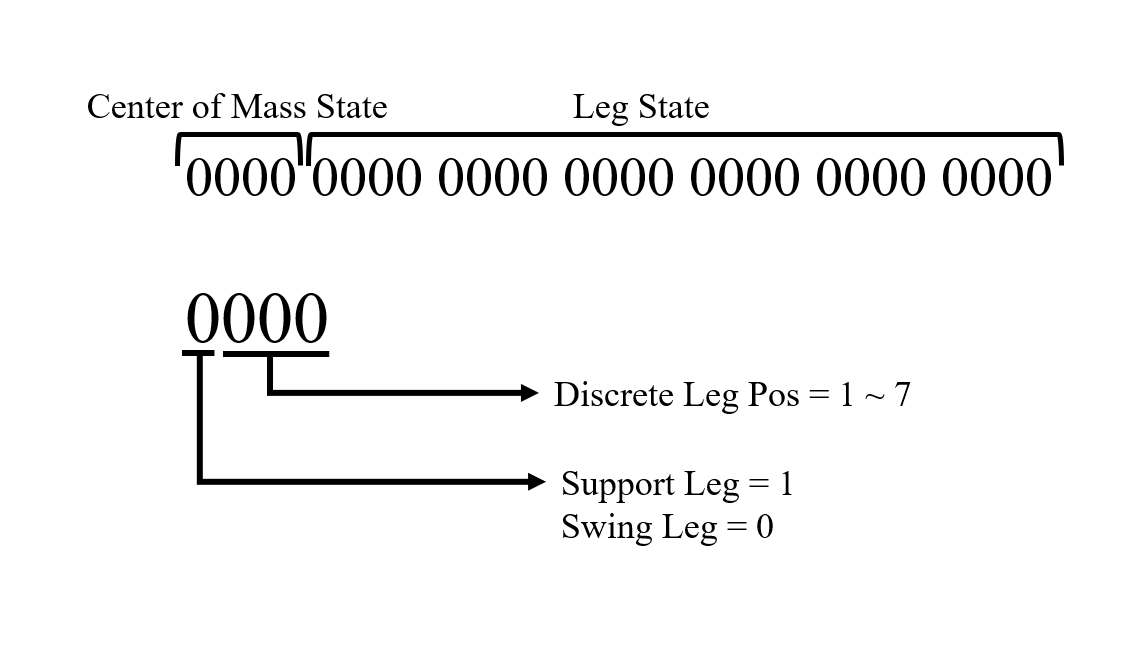
\includegraphics[width=90mm, clip]{figure/chapter3/leg_state.png}
    \caption{Leg State Bit}
    \label{fig:leg_state_bit} % chktex 24
  \end{center}
\end{figure}

\section{歩容パターンの再評価手法の実装}

\section{グラフ探索による自由歩容パターン生成手法の統合}
先行研究において,グラフ探索による自由歩容パターン生成手法はロボットの動作によって別のものを使用しており,
それぞれ別のプログラムで実装されている.
不整地の踏破を行うためには,さまざまな動作を組み合わせて使用する必要がある.
そのため本研究では,グラフ探索による自由歩容パターン生成手法を統合し,
1つのプログラムで実行できるようにした.

\subsection{ロボットの動作}
先行研究において,すでに実装されているロボットの動作を表\ref{tab:ロボットの動作}に示す.
表において,2次元空間とはロボットが平面上で動作することを表し,
3次元空間とはロボットが立体的な地形で動作することを表す.

\begin{table}[htbp]
	\caption{実装済みのロボットの動作}
	\label{tab:ロボットの動作}  % chktex 24
	\begin{center}
   	\begin{tabular}{|c|c|c|c|c|c|c|} \hline  % chktex 44
    	\backslashbox{動作}{ロボット} & 2次元空間 & 3次元空間  \\ \hline  % chktex 44
      直進 & $\bigcirc$ & $\bigcirc$ \\ \hline  % chktex 44
      その場旋回 & $\bigcirc$ & $\times$ \\ \hline  % chktex 44
      旋回 & $\bigcirc$ & $\times$ \\ \hline  % chktex 44
      旋回 & $\bigcirc$ & $\times$ \\ \hline  % chktex 44
      特定姿勢での静止 & $\bigcirc$ & $\times$ \\ \hline  % chktex 44
      %% まるはtexにおいて,$\bigcirc$
      %% ばつはtexにおいて,$\times$
    \end{tabular}
  \end{center}
\end{table}

\subsection{自由歩容パターン生成手法の切り替えアルゴリズム}
